\documentclass[12pt,a4paper]{report}

% --- Encodage et langues ---
\usepackage[utf8]{inputenc}
\usepackage[T1]{fontenc}
\usepackage[french]{babel}

% --- Mathématiques ---
\usepackage{amsmath, amsfonts, amssymb}

% --- Graphiques et images ---
\usepackage{graphicx}
\usepackage{caption}
\usepackage{float}

% --- Code source ---
\usepackage{listings}

% --- Mise en page ---
\usepackage{geometry}
\usepackage{fancyhdr}
\usepackage{setspace}

% --- Symboles ---
\usepackage{eurosym}

% --- Couleurs ---
\usepackage{xcolor}

% --- Hyperliens ---
\usepackage{hyperref}
\hypersetup{
    colorlinks=true,
    linkcolor=blue,
    urlcolor=blue,
    citecolor=blue
}

% --- Marges ---
\geometry{top=2cm, bottom=2cm, left=2cm, right=2cm}

% --- En-tête et pied de page ---
\pagestyle{fancy}
\fancyhead[L]{3\textsuperscript{ème} année}
\fancyhead[C]{\small \nouppercase{\leftmark}}
\fancyhead[R]{2025-2026}
\fancyfoot[C]{\thepage}

% --- Interlignes ---
\setstretch{1}

\begin{document}

% --- Page de garde ---
\begin{titlepage}

    \begin{figure}[htbp]
        \centering
        \includegraphics[width=0.2\textwidth]{images/logo CYECH.JPG} 
        \hspace{10cm}
        
\includegraphics[width=0.1\textwidth]{images/logo AFI24.png}
    \end{figure}

    \vspace{0.5cm}

    \begin{center}
        \huge{\textbf{RAPPORT:}} \\
        \vspace{0.5cm}
        \Large{\textbf{ARBRE BINOMIAL}}\\
        \vspace{1cm}
        \textbf{Encadré par: Mme } \\
        \textbf{Matière: MATHEMATIQUES POUR LA FINANCE} \\
    \end{center}

    \vspace{2cm}

    \textbf{Réalisé par :}
    \begin{itemize}
        \item Charly-Romy TANGA
    \end{itemize}

    \vspace{1cm}
    \begin{center}
        \Large{\textbf{CY TECH}} \\
        \vspace{0.3cm}
        \large{Ingénieur 3\textsuperscript{ème} année \\ INGÉNIEUR MATHÉMATIQUES OPTION FINANCE ET TECHNOLOGIE } \\
    \end{center}
    \begin{center}
        Année Universitaire : 2025-2026
    \end{center}

\end{titlepage}

\clearpage
\hypersetup{pageanchor=true}

% --- Table des matières ---
\tableofcontents

\clearpage
\chapter*{Introduction}
\addcontentsline{toc}{chapter}{Introduction}

\section*{Contexte}
\section*{Espace de probabilité sans risque neutre}
L'évaluation de la prime de l'option $V_0$ repose sur l'idée d'un \textbf{espace de probabilité neutre au risque}.  
On définit la probabilité neutre $q$ par :

\[
q = \frac{(1+r) - d}{u - d}
\]

Cette probabilité permet de calculer l'espérance \textit{actualisée} des flux futurs de l'option, dans un monde sans arbitrage.

avec :  
\begin{itemize}
    \item $u$ : facteur de hausse  
    \item $d$ : facteur de baisse  
    \item $r$ : taux sans risque par période  
    \item $q = \frac{(1+r)-d}{u-d}$ : probabilité neutre au risque  
\end{itemize}
\section*{Lien avec la couverture et le théorème fondamental}
La valeur initiale de l'option $V_0$ peut être déterminée en construisant un portefeuille \textbf{couvert}, combinant l'actif sous-jacent et une position sans risque.  
Cette méthode garantit que le prix de l'option respecte le \textbf{théorème fondamental de la valorisation} et ne permet pas de profiter d'une \textbf{opportunité d'arbitrage}.

Une \textbf{option} dans le modèle binomial est un produit dérivé dont la valeur dépend du prix de l'actif sous-jacent.  
On considère la forme dynamique suivante pour une option européenne  :

\[
V_{n,i} = \frac{1}{1+r} \, \mathbb{E}^{\mathbb{Q}}\big[ V_{n+1} \mid \mathcal{F}_n \big]
= \frac{1}{1+r} \Big[ q \, V_{n+1,i+1} + (1-q) \, V_{n+1,i} \Big]
\]


où :  
\begin{itemize} 
    \item $\mathbb{E}^{\mathbb{Q}}[\cdot \mid \mathcal{F}_n]$ : espérance conditionnelle sous la probabilité neutre au risque $q$  
    \item $V_{n+1,i+1}, V_{n+1,i}$ : valeurs futures de l'option selon l’état up/down  
    \item $1/(1+r)$ : actualisation à la période précédente  
    \item $V_{n,i}$ : valeur de l'option à l'étape $n$, état $i$
\end{itemize}

Le \textbf{delta} au nœud $(i,j)$ se calcule par :  
\[
\Delta_{i,j} = \frac{V_{i+1,j+1} - V_{i+1,j}}{S_{i+1,j+1} - S_{i+1,j}}
\]

Pour illustrer, on considère $T=2$ périodes et $N=2$ étapes. L'objectif est de construire l'arbre binomial et de calculer $V_0$, $V_2$, ainsi que $\Delta$ à chaque nœud.  

\clearpage
\chapter*{Pseudo-code}
\addcontentsline{toc}{chapter}{Pseudo-code}

\begin{lstlisting}[language=Python, basicstyle=\ttfamily\small]
# Paramètres : S0, K, r, u, d, T, N, option_type
# Initialisation
dt = T / N
R = exp(r*dt)
p = (R - d)/(u - d)
# Arbre des prix du sous-jacent
S = zeros((N+1, N+1))
for i in range(N+1):
    for j in range(i+1):
        S[j,i] = S0 * u**j * d**(i-j)
# Arbre des valeurs de l'option à maturité
V = zeros_like(S)
for j in range(N+1):
    if option_type == 'call':
        V[j,N] = max(S[j,N] - K, 0)
    else:
        V[j,N] = max(K - S[j,N], 0)
# Récurrence backward pour V
for i in range(N-1, -1, -1):
    for j in range(i+1):
        V[j,i] = (p*V[j+1,i+1] + (1-p)*V[j,i+1])/R
# Calcul du delta au nœud (i,j)
Delta = NaN * ones_like(S)
for i in range(N):
    for j in range(i+1):
        Delta[j,i] = (V[j+1,i+1] - V[j,i+1]) / (S[j+1,i+1] - S[j,i+1])
# Résultat : S, V, Delta, V0, Delta0, V2
\end{lstlisting}

\clearpage
\chapter*{Sorties}
\addcontentsline{toc}{chapter}{Sorties}

% --- Arbre complet ---
\begin{figure}[H]
    \centering
    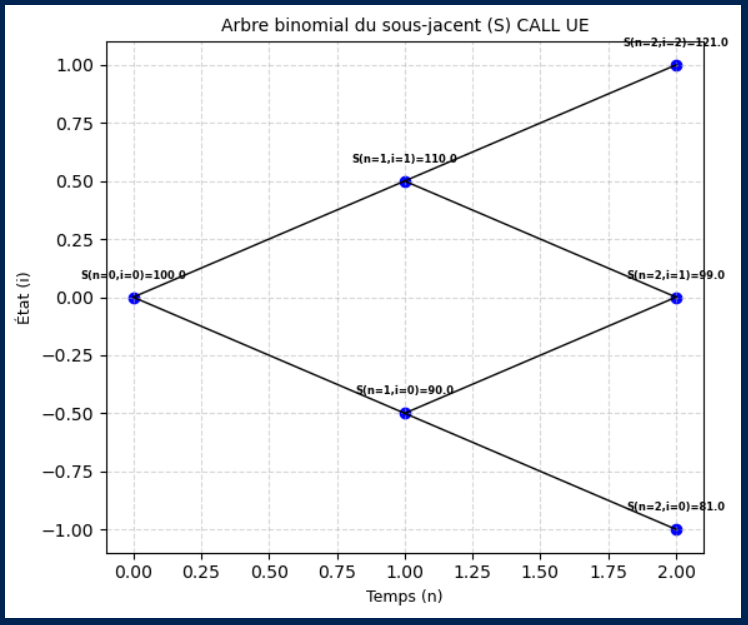
\includegraphics[width=0.8\textwidth]{images/arbres_call.PNG}
    \caption{Arbre complet : prix du sous-jacent (S), valeurs de l'option (V) et Delta à chaque nœud pour le CALL}
\end{figure}
\begin{figure}[H]
    \centering
    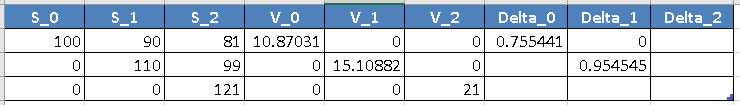
\includegraphics[width=0.8\textwidth]{images/Tableau_complet_CALL.PNG}
    \caption{Tableau complet : prix du sous-jacent (S), valeurs de l'option (V) et Delta à chaque nœud pour le CALL}
\end{figure}

% --- Résumé des valeurs importantes ---
\begin{figure}[H]
    \centering
    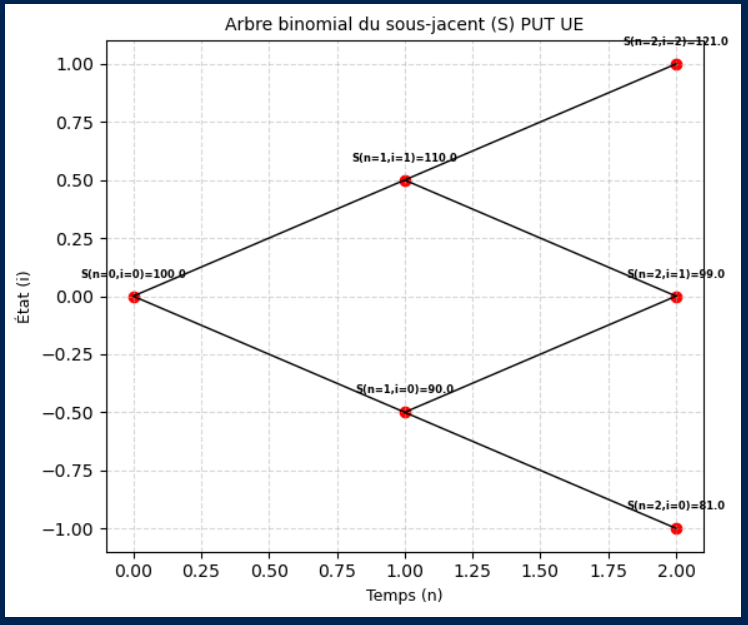
\includegraphics[width=0.8\textwidth]{images/arbres_put.PNG}
    \caption{Arbre complet : prix du sous-jacent (S), valeurs de l'option (V) et Delta à chaque nœud pour le PUT}
\end{figure}
\begin{figure}[H]
    \centering
    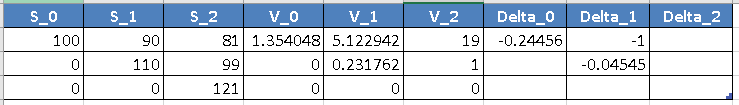
\includegraphics[width=0.8\textwidth]{images/Tableau_complet_PUT.PNG}
    \caption{Tableau complet : prix du sous-jacent (S), valeurs de l'option (V) et Delta à chaque nœud pour le PUT}
\end{figure}

\clearpage
\chapter*{Annexes}
\addcontentsline{toc}{chapter}{Annexes}

% Contenu du code complet (captures d'écran)
\begin{figure}[H]
    \centering
    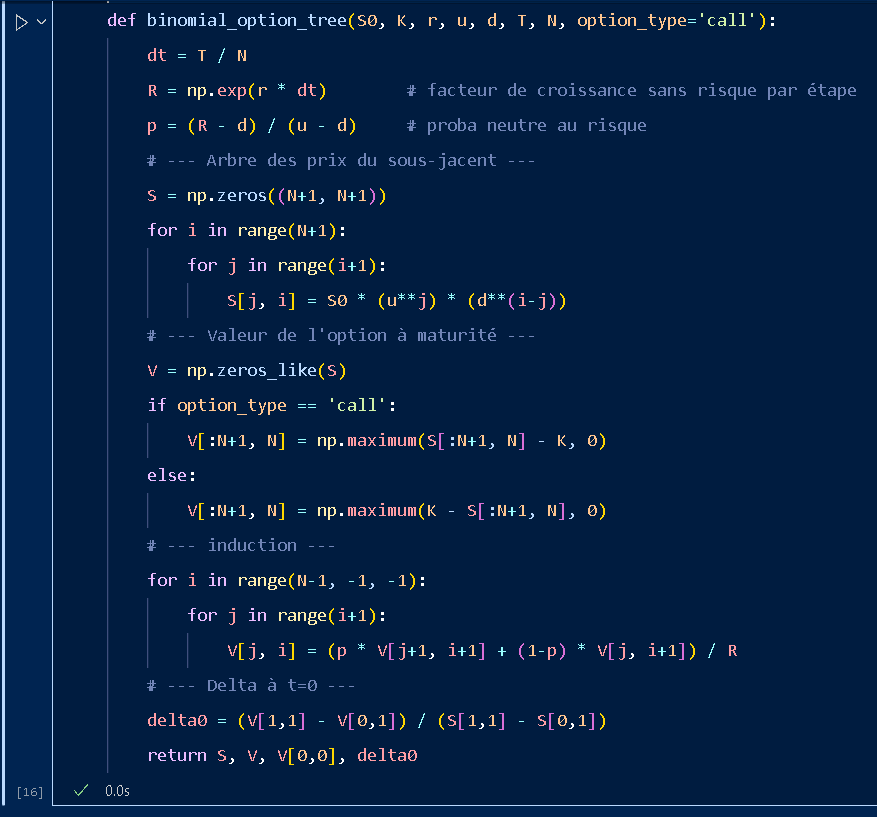
\includegraphics[width=0.8\textwidth]{images/code_Pythin_Option_Modele_Binomial.png}
    \caption{Code Python complet pour l'option}
\end{figure}

\end{document}
